\section{Data association}

When using factor graphs to solve the SLAM problem, an important thing to think about is how the measurements are associated to the right landmark. This is relatively easy when you do feature-based SLAM, e.g. when you use a visual slam system like ORB-SLAM \cite{ORBSLAM}. This is because the measurement itself has a direct way of being compared with other features for how alike they are, and a single point in space is usually pretty distinct. \\

This is however not the case with the detection systems employed on Revolves race car. Since the cones are very similar, a feature extracting algorithm was not thought to work, and all the detections systems only give out a position in the plane, with the camera system outputting a cone color as well. This means the SLAM system needs to be able to keep track of which measurements are to the same cone, or landmark as it's usually referred to when talking about SLAM. \\

\subsection{Last years solution}

Last year this was done with a very naive algorithm, that simply said that if a new detection was within a certain radius from an existing cone in the exisitng map, it was the same cone. If a measurement could not be associated to the existing map, it had to be seen above a certain number of times to be added to the map. This meant that the system had a list of hypothesises that a new measurement was associated to the same way it was associated to the map. \\ 

This method did however not take into account the different spatial uncertainties stemming from the different detection algorithms, nor did it account for the varying uncertainty of the state estimation. It also didn't have a way of distrusting the landmarks if it hadn't been seen when it should have been. \\

\subsubsection{Previous work} \todo{Remove title previous work?}

Most of the work done on data association is used for object tracking, typically using a radar\cite{RadarTracking}, but also more recently been used to track visually\cite{VisualTracking}. Data association used for tracking implies finding out which of the tracked objects correspond to new measurements, where typically the measurements are all made from a stationary vantage point, while the objects are moving around. This means one must predict where the objects are going to be and try to match all observed objects with objects that are being tracked. \\

Data association applied to SLAM have been more common in the recent years. It is an almost opposite problem to the tracking problem, as the observer is the one moving around, while the landmarks are standing still. While a lot of the work done on tracking focuses on single or a handfull of objects to track, when solving the SLAM problem one by definition want to be able to handle a large amount of landmarks. This is because the output of the system is going to be the map, and you want it to be able to handle all the landmarks that build up the map. The data association problem met in the two settings are however quite similar, and work done in one field therefore benefits the other. \\

\subsection{Nearest Neighbour}

When talking about the data assocation problem and its solutions it's essential to keep in mind at all times what application is being discussed. In many of the earlier cases the tracking problem is simply matching measurements with one object, in which case a nearest neighbor matching with the Malahanobis distance can work wonders\cite{ShalomTracking}. \\ 

In this case it is assumed that one of the measurements is the object, and you're simply trying to know which one it most likely is. It's assumed that the objects movement can be approximated as

\begin{equation}
    p_{next} = Ap_{prev} + w_{model}
\end{equation}

That is then measured with a measurement model

\begin{equation}
    p_{meas} = Hp_{true} + w_{meas}
\end{equation}
 
Here A is the linearized dynamic model for how the object moves, H is the linearized measurement function and $w_{model}$ and $w_{meas}$ are additive zero-mean white noise for the model and measurement, respectively. It then uses a Kalman filter step to propagate the expected position and covariance of the object using the previous position, the dynamic model of the object and a covariance for both the previous position and the dynamic model. This then gives the new estimated position of the object and it's covariance. Using the estimated and measured positions and covariances, the nearest neighbor is then found using the Mahalanobis distance\cite{MahalanobisTracking}:

\begin{equation}
    d^2_{Mahala} = (p_{est} - p_{meas})^T(\Sigma_{est} - \Sigma_{meas})^{-1}(p_{est} - p_{meas})
\end{equation}

The Mahalanobis distance can be seen as a scaled euclidian distance, where the reference frame is rotated to match the principal axes of the distribution and the axes are scaled to the variance along the principal axes of the distribution. This means that a unit length in the euclidian sense is larger if it is in a direction where the variance is small and vice versa. The height curves of the Gaussian and its principal axes are illustrated in figure \ref{Fig:GaussianPrincipalAxes}. \\

\begin{figure}
    \centering
    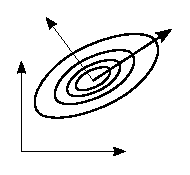
\includegraphics[width=0.5\linewidth]{0_Images/3_Theory/GaussianPrincipalAxis.eps}
    \captionof{figure}{Height curves of a Gaussian distribution, with its principal axes.}
    \label{Fig:GaussianPrincipalAxes}
\end{figure}

\subsection{Probabilistic Data Association Filter}

The problem with the above method is that, even when the dynamics of the object and the measurement function are in fact linear and known perfectly, there is a non-zero probability that the measurement used to update the object is the wrong measurement, in which case track might be lost. A more sophisticated approach that tracks one target in in the presence of false alarms and low probability of detection at each time step, is \cite{BarShalomPDA}. Instead of assigning one measurement to the object at each instant, they use all the validated measurements to update the object, weighting each measurement with probabilities that they actually are from the object.  \\

Much like the nearest neighbour association, it assumes a known linear state transition with additive white noise

\begin{equation}
    x_{k+1} = F_kx_k + w_k, k=0,1,2..
\end{equation}

where $F_k$ is known, $w_k$ has zero mean and a known variance of 

\begin{equation}
    E(w_kw_j') = Q_k\delta_{kj}
\end{equation}

Note that knowing the transition matrix means the tracked object is non-maneuvering. The initial state is assumed normally distributed with mean $\hat{x}_{0|0}$ and covariance $P_{0|0}$, independent of $w_k$. Similarily it is assumed a known linear measurement function with additive white noise

\begin{equation}
    z_k = H_kx_k + y_k, k = 1,2,..
\end{equation}

where $H_k$ is known and $y_k$ is the measurement noise with zero mean known variance 

\begin{equation}
    E(v_kv_j') = R_k\delta_{kj}
\end{equation}

\\

Furthermore it assumes a validation method that guarantees that the correct measurement will be kept with a certain probability. It also assumes that the false positives are spatially uniform and independent. The number of false positives at each time instant is not known exactly.   \\ 

The validation method used is to reject measurement $i$ if it doesn't pass the test

\begin{equation}
    \nu_{k,i}'S_k^{-1}\nu_{k,i} \leq \gamma
\end{equation}

where 

\begin{equation}
    S_k = H_kP_{k|k-1}H'_k+R_k
\end{equation}

and $\nu_{k,i} = z_{k,i} - \hat{z}_{k|k-1}$ is the difference between measurement $z_{k,i}$ and the predicted object position $\hat{z}_{k|k-1}$ at time step $k$. $\gamma$ is the validiation gate threshold. This assures that the correct measurement will be kept with a certain probability. \\

The linearity assumptions added above is later removed and accounted for by increasing the covariances on the state transition and measurement. Each validated measurement is used to update the object position, and it is shown on a highly nonlinear simulation problem that the resulting track is better than both the nearest neighbour filter and a track splitting filter, where each new measurement spawns a new filter. The latter is exponential in the number of false positives, so is very unfeasible in many situations. 

\subsection{Joint Probabilistic Data Association}

To handle the more useful case of having more than one object to track in the presence of uniform poisson clutter, the Joint Probabilistic Data Association (IPDA) method was developed\cite{JPDA}. It assumes several objects, uniformly distributed clutter in the neighborhood of the objects and low probabilities of detecting the targets at each time step. When the targets are far enough away that none of the same measurements are possible to associate to both, the algorithm is like running several PDAF's in parallell. However, when measurements are possible to associate to more than one target, JPDA takes this into account. \\ 

This leads to good tracking, but at the cost of a much higher computational cost, especially when there are many targets. In addition it assumes the number of targets are known, and has no logic to intitialize and terminate possible tracks. This is dealt with in \cite{Multitrack}. In \cite{JPDARev} the $M$ best possible permutations of measurement to target matches are found using Linear Programming (LP). This leads to a massive reduction in runtime compared with the pure JPDA, while retaining most of the performance. Like with the JPDA it does not handle initializing and terminating tracks. \\

\subsection{Joint Maximum Likelihood}

In the domain of data association for SLAM, a valid option that must be mentioned is the Joint Maximum Likelihood (JMH)\cite{JMH}. It aims to solve the problem of uniquely associating a batch of measurements of landmarks to existing landmarks. It does this by finding the set, $E_k = \{ e_1, e_2, ... , e_m\} $, of associations, where each $e_n = {i,j}$ represents an association between measurement $i$ and landmark $j$. This is done by finding the set of data associations that maximizes the products of likelihoods

\begin{equation}
    E_k = \argmax_{E_l} \prod_{\forall e_m \in E_l} f_{e_{i,j}}
\end{equation}

where 

\begin{equation}
    f_{i,j} = \frac{1}{(2\pi)^{n/2}} exp(-\frac{1}{2}\nu_{i,j}^T\delta_j^{-1}\nu_{i,j})
\end{equation}

To avoid overflow this is transformed into maximizing the sum of the log-likelihoods instead.

\begin{equation}
    E_k = \argmax_{E_l} \sum_{\forall e_m \in E_l} ln(f_{em})
\end{equation}

which is then the same as finding the $E_l$ that minimizes the Malahanobis distance.

\begin{equation}
    E_k = \argmin_{E_l} \sum_{\forall e_m \in E_l} N_{e_m}
\end{equation}

where 

\begin{equation}
    N_{e_m} = \nu_{i,j}^TS_j^{-1}\nu_{i,j} 
\end{equation}

\subsection{Joint Compatibility}

Doing almost the same as the JMH, but instead of minimizing the normalized distances, one aims to find a set that gives as many measurement-landmark associations that satisfy the compatibility test

\begin{equation}
    \nu_{i,j}^TS_j^{-1}\nu_{i,j} \leq \gamma_n
\end{equation}

as possible. Here $\gamma_n$ is usually taken to be around $0.95$, i.e. that it's $\SI{95}{\percent}$ probable that measurement $i$ came from landmark $j$. This problem is known as Joint Compatibility, and one solution is found in \cite{Bailey}

\subsection{Simplifications of the Data association problem for Formula Student}

The data association problem Revolve NTNU faces when making a driverless car for Formula Student differes in a few ways from the problems solved in the literature. The main difference lies in that it's possible to add more restraints on the problem. The positions of the landmarks are quite regular, the rules stating that they should never be more than \SI{5}{\meter} between consecutive cones on either side, and the track width is never less than \SI{3}{\meter}. The cones aren't too spaced too close either. The latter is not stated explicitly in the rules, but is known by looking at the videos of the events from previous years. \\ 

The problem is also simplified by looking at data from the detection algorithms. First of all the false positives that arrive aren't random false positives, but rather objects or walls in the viscinity of the track that aren't cones. This means they all lie outside of the track and therefore aren't too dangerous if they enter into the map. \\

Secondly the false postives that stem from walls or large objects aren't constant in position. This is taken advantage of by having new possible landmarks have to be verified more than once before being accepted, and every time a hypothesis doesn't get a new association it's confidence is decremented. This means that a wall will spawn new landmarks along it that then decay in confidence and eventually get discarded, as long as we aren't unlucky and get enough measurements to almost the same spot. Experiments tell us that this isn't a problem. \\ 

Lastly it is possible to take advantage of the fact that the different detection algorithms have different false positive rates. The camera for example barely ever accepts a false positive, but has a rather large error in the position of the detected cone. This is also used to our benefit, as will be explained below. 
